\documentclass[a4paper,titlepage,11pt,twosides,floatssmall]{mwrep}
\usepackage[left=2.5cm,right=2.5cm,top=2.5cm,bottom=2.5cm]{geometry}
\usepackage[OT1]{fontenc}
\usepackage{polski}
\usepackage{amsmath}
\usepackage{amsfonts}
\usepackage{amssymb}
\usepackage{graphicx}
\usepackage{float}
\usepackage{url}
\usepackage{tikz}
\usetikzlibrary{arrows,calc,decorations.markings,math,arrows.meta}
\usepackage{rotating}
\usepackage[percent]{overpic}
\usepackage[cp1250]{inputenc}
\usepackage{xcolor}
\usepackage{colortbl}
\usepackage{pgfplots}
\usetikzlibrary{pgfplots.groupplots}
\usepackage{listings}
\usepackage{matlab-prettifier}
\usepackage{enumitem,amssymb}
\definecolor{szary}{rgb}{0.95,0.95,0.95}
\usepackage{siunitx}
\usepackage{gensymb} %do st. Celsjusza
\usepackage{graphicx} %do załączania png
\sisetup{detect-weight,exponent-product=\cdot,output-decimal-marker={,},per-mode=symbol,binary-units=true,range-phrase={-},range-units=single}
\SendSettingsToPgf
%konfiguracje pakietu listings
\lstset{
	backgroundcolor=\color{szary},
	frame=single,
	breaklines=true,
}
\lstdefinestyle{customlatex}{
	basicstyle=\footnotesize\ttfamily,
	%basicstyle=\small\ttfamily,
}
\lstdefinestyle{customc}{
	breaklines=true,
	frame=tb,
	language=C,
	xleftmargin=0pt,
	showstringspaces=false,
	basicstyle=\small\ttfamily,
	keywordstyle=\bfseries\color{green!40!black},
	commentstyle=\itshape\color{purple!40!black},
	identifierstyle=\color{blue},
	stringstyle=\color{orange},
}
\lstdefinestyle{custommatlab}{
	captionpos=t,
	breaklines=true,
	frame=tb,
	xleftmargin=0pt,
	language=matlab,
	showstringspaces=false,
	basicstyle=\footnotesize\ttfamily,
	%basicstyle=\scriptsize\ttfamily,
	keywordstyle=\bfseries\color{green!40!black},
	commentstyle=\itshape\color{purple!40!black},
	identifierstyle=\color{blue},
	stringstyle=\color{orange},
}

%wymiar tekstu (bez zywej paginy)
\textwidth 160mm \textheight 247mm

%ustawienia pakietu pgfplots
\pgfplotsset{
tick label style={font=\scriptsize},
label style={font=\small},
legend style={font=\small},
title style={font=\small}
}

\def\figurename{Rys.}
\def\tablename{Tab.}

%konfiguracja liczby plywajacych elementow
\setcounter{topnumber}{0}%2
\setcounter{bottomnumber}{3}%1
\setcounter{totalnumber}{5}%3
\renewcommand{\textfraction}{0.01}%0.2
\renewcommand{\topfraction}{0.95}%0.7
\renewcommand{\bottomfraction}{0.95}%0.3
\renewcommand{\floatpagefraction}{0.35}%0.5

\begin{document}
\frenchspacing
\pagestyle{uheadings}

%strona tytulowa
\title{\bf Sprawozdanie z projektu i cwiczenia laboratoryjnego nr 1, zadanie nr 2\vskip 0.1cm}
\author{Eva Reszka, Mateusz Roszkowski,  Dominika Zajac}
\date{2021}

\makeatletter
\renewcommand{\maketitle}{\begin{titlepage}
\begin{center}{\LARGE {\bf
Wydzial Elektroniki i Technik Informacyjnych}}\\
\vspace{0.4cm}
{\LARGE {\bf Politechnika Warszawska}}\\
\vspace{0.3cm}
\end{center}
\vspace{5cm}
\begin{center}
{\bf \LARGE Projektowanie ukladow sterowania\\ (projekt grupowy) \vskip 0.1cm}
\end{center}
\vspace{1cm}
\begin{center}
{\bf \LARGE \@title}
\end{center}
\vspace{2cm}
\begin{center}
{\bf \Large \@author \par}
\end{center}
\vspace*{\stretch{6}}
\begin{center}
\bf{\large{Warszawa, \@date\vskip 0.1cm}}
\end{center}
\end{titlepage}
}
\makeatother

\maketitle

\tableofcontents
% !TEX encoding = cp1250
\chapter{Wst�p}

mozna napisac glupoty albo mozna wyrzucic
% !TEX encoding = cp1250
\chapter{Projekt}



\section{Sprawdzenie poprawno�ci punktu pracy}

Implementacja zadania znajduje si� w pliku \texttt{zad1\_2.m}.

Punkt pracy r�wny jest $U_{pp} = 0$, $Y_{pp} = 0$, co zosta�o przedstawione na wykresach \ref{zad1_u} i \ref{zad1_y}.

\begin{figure}[H]
	\centering
	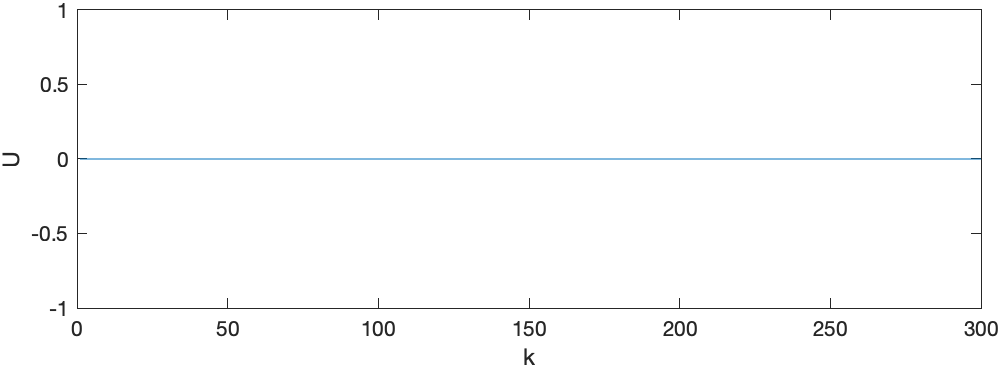
\includegraphics[scale=0.75]{png/projekt/zad1_u.png}
	\caption{Wej�cie uk�adu w punkcie pracy}
	\label{zad1_u}
\end{figure}

\begin{figure}[H]
	\centering
	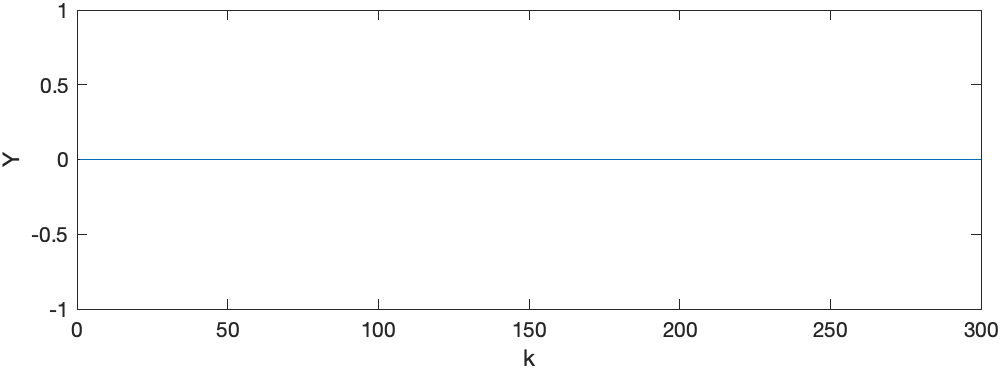
\includegraphics[scale=0.75]{png/projekt/zad1_y.png}
	\caption{Wyj�cie uk�adu w punkcie pracy}
	\label{zad1_y}
\end{figure}

 
\section{Wyznaczenie odpowiedzi skokowych procesu}

Uk�ad zosta� pobudzony sygna�ami o warto�ciach $ U = [-0,8; -0,3; 0,2; 0,6; 1,0]$.

Otrzymane zosta�y w ten spos�b odpowiedzi skokowe:

\begin{figure}[H]
	\centering
	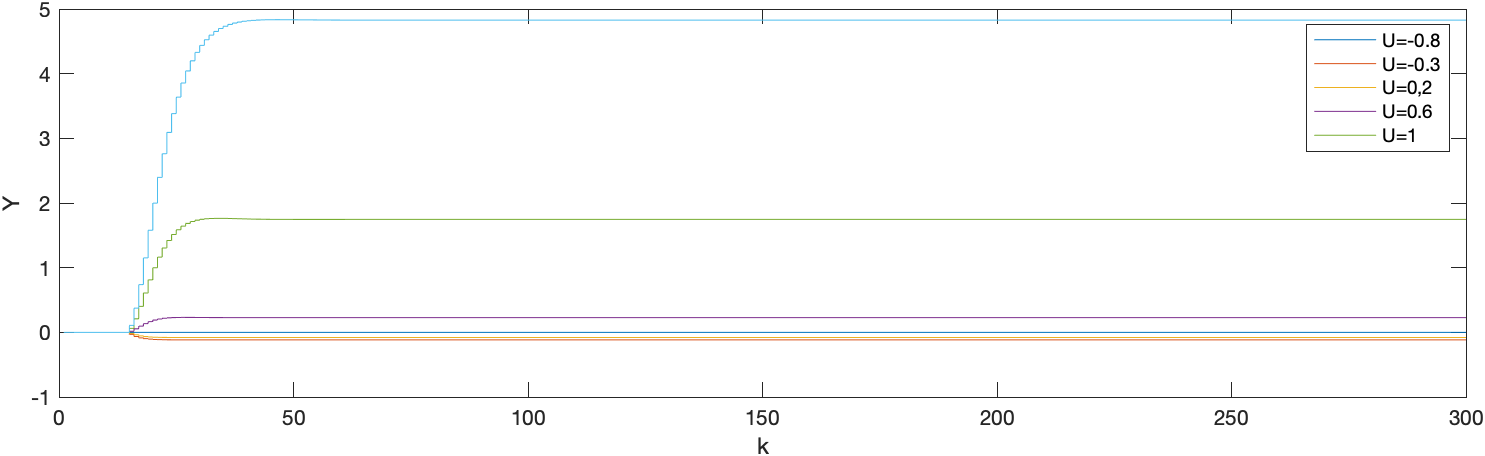
\includegraphics[scale=0.6]{png/projekt/zad2_1.png}
	\caption{Otrzymane odpowiedzi skokowe}
	\label{zad2_1}
\end{figure}

Na wykresie  \ref{zad2_2}  widoczna jest charakterystyka statyczna obiektu.

\begin{figure}[H]
	\centering
	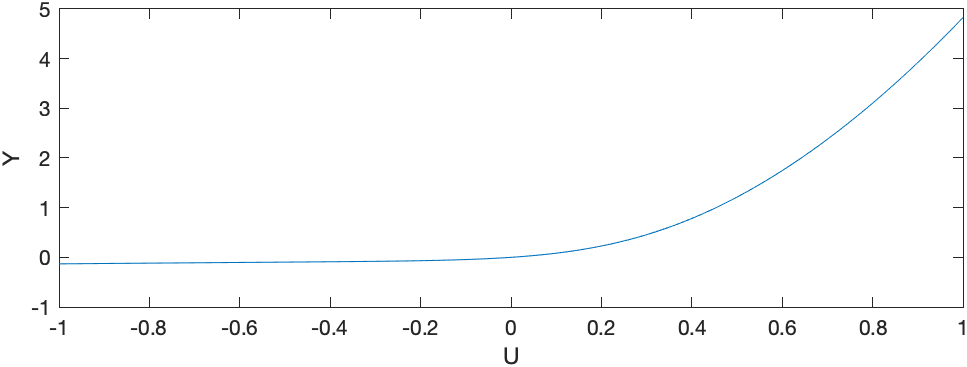
\includegraphics[scale=0.75]{png/projekt/zad2_2.png}
	\caption{Charakterystyka statyczna}
	\label{zad2_2}
\end{figure}

W�a�ciwo�ci dynamiczne oraz statyczne nie s� liniowe. Do charakterystyki statycznej nie mo�e zosta� dopasowana prosta.

\section{Algorytmy PID i DMC}

Obiekt zosta� poddany regulacji za pomoc� algorytm�w PID i DMC z Projektu 2.

TODO opis PID, DMC

\begin{figure}[H]
	\centering
	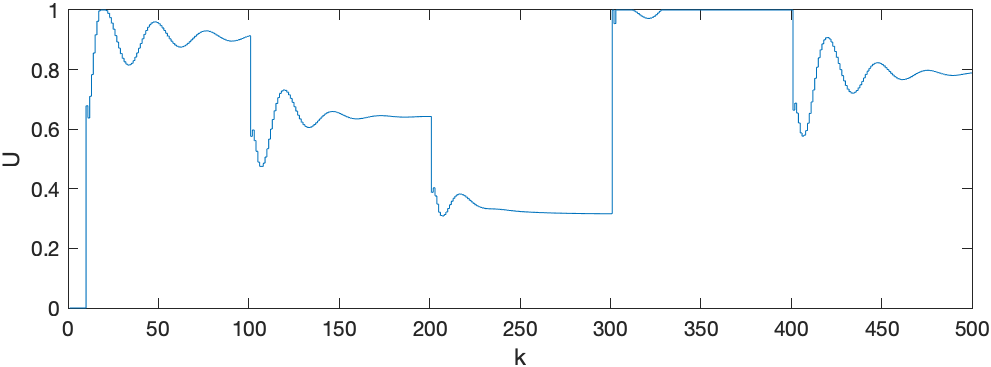
\includegraphics[scale=0.75]{png/projekt/zad3_pid_u.png}
	\caption{Wej�cie uk�adu - algorytm PID}
	\label{zad3_pid_u}
\end{figure}

\begin{figure}[H]
	\centering
	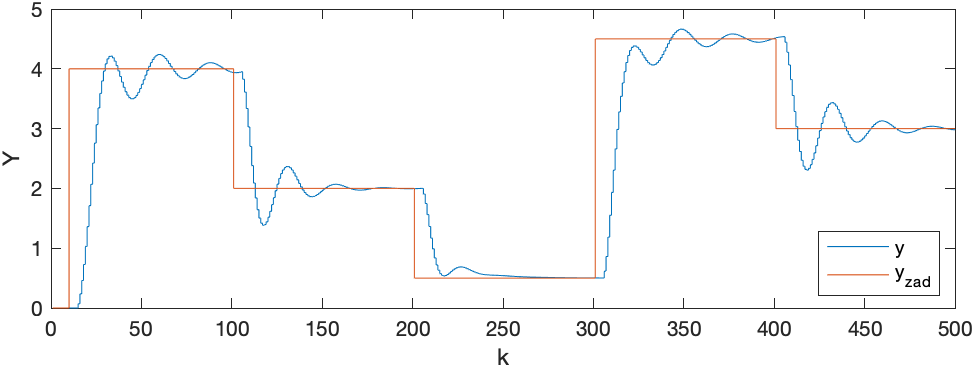
\includegraphics[scale=0.75]{png/projekt/zad3_pid_y.png}
	\caption{Wyj�cie uk�adu - algorytm PID}
	\label{zad3_pid_y}
\end{figure}

\begin{figure}[H]
	\centering
	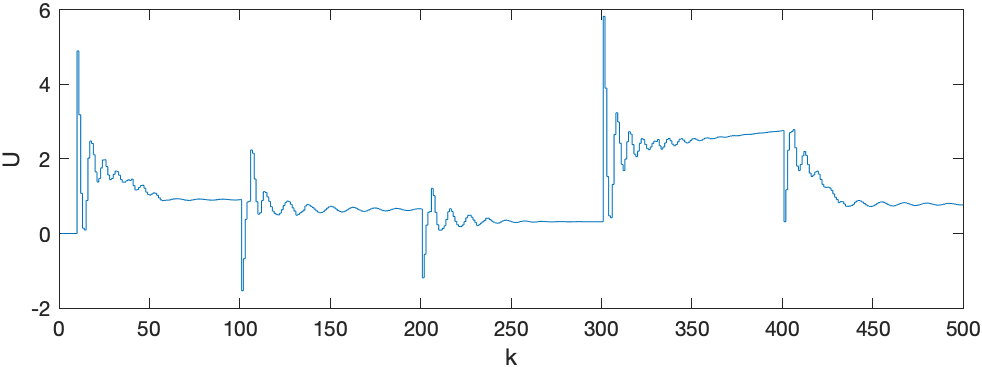
\includegraphics[scale=0.75]{png/projekt/zad3_dmc_u.png}
	\caption{Wej�cie uk�adu - algorytm PID}
	\label{zad3_dmc_u}
\end{figure}

\begin{figure}[H]
	\centering
	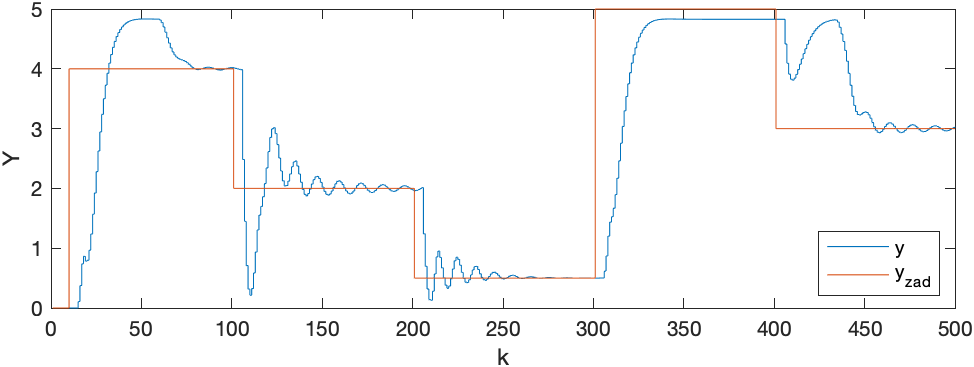
\includegraphics[scale=0.75]{png/projekt/zad3_dmc_y.png}
	\caption{Wyj�cie uk�adu - algorytm PID}
	\label{zad3_dmc_y}
\end{figure}



\section{Rozmyty algorytm PID}

\section{Rozmyty algorytm DMC}


% !TEX encoding = cp1250
\chapter{�wiczenie laboratoryjne}

Podczas tego zadania laboratoryjnego wykorzystano:
\begin{itemize}
	\item grza�k� G1 (sygna� steruj�cy $U$),
	\item wentylator W1 (warto�� zadana $Y_{zad}$),
	\item czujnik temperatury T1 (sygna� wyj�ciowy $Y$) 
\end{itemize} 

\section{Przygotowanie do wykonania �wiczenia}
Przed rozpocz�ciem pomiar�w sprawdzono mo�liwo�� sterowania i~pomiaru w~komunikacji ze stanowiskiem. Punkt pracy grza�ki $G1$ dla zespo�u obliczony zosta� wg. wzoru \ref{w_G1}:
\begin{equation}
	G1 = 25 + Z\%5\
\label{w_G1}
\end{equation}
gdzie Z~to numer zespo�u, zatem dla naszego zespo�u Z02 punkt pracy wynosi:
\begin{equation}
	G1 = 25 + 2\%5 = 27
\end{equation}
Nast�pnie okre�lono warto�� pomiaru temperatury T1 dla obliczonego punktu pracy. W~tym celu moc wentylatora W1 ustawiono na 50\%, a moc grza�ki G1 na 27\%,  za pomoc� funkcji
\texttt{sendControls([1,5], [50,27])}.
Warto�� pomiaru temperatury odczytano korzystaj�c z~funkcji 
\texttt{readMeasurements(1)}.
Temperatura T1 ustabilizowa�a si� na warto�ci \textbf{32.25\degree C}

 
\section{Wyznaczenie odpowiedzi skokowych procesu}
Zarejestrowano przebieg temperatury T1 dla trzech r�nych zmian sygna�u steruj�cego G1 rozpoczynaj�c z~punktu pracy (27\%) do 10\%, 35\% i~50\%.
Otrzymane przebiegi zmian przedstawiono na Rys. \ref{rys_przebiegi_T1}. 

\textcolor{red}{
	Czy w�a�ciwo�ci statyczne obiektu mo�na okre�li� jako (w przybli�eniu) liniowe? Je�li tak wyznaczy� wzmocnienie statyczne procesu?
}

\newpage
\begin{figure}[H]
	\centering
	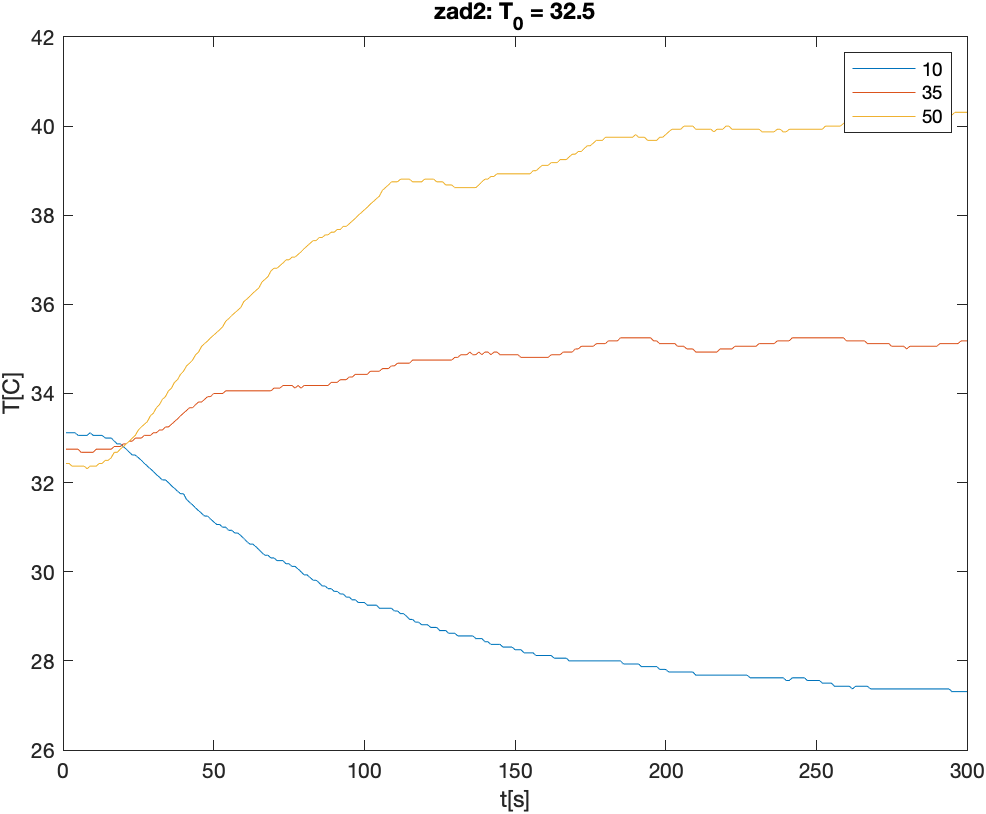
\includegraphics[scale=0.35]{png/lab1_zad2.png}
	\caption{Odpowiedzi skokowe procesu}
	\label{rys_przebiegi_T1}
\end{figure}

\section{Algorytm PID}

Poni�sze zadanie laboratoryjne realizowane by�o w inny, zimniejszy dzie�, co spowodowa�o konieczno�� wyznaczenia warto�ci pomiaru temperatury w punkcie pracy na nowo. Nowy punkt pracy dla ${G1 = 27}$ to ${ T1 = 29.37 }$ {\degree C}.

Napisano  program do regulacji cyfrowego algorytmu PID. Dob�r nastaw regulatora przeprowadzono metod� Zieglera-Nicholsa. Rozpocz�to od doboru warto�ci wzmocnienia K, przy parametrze ca�kuj�cym Ti = inf i r�niczkuj�cym Td = 0. W algorytmie uwzgl�dniono ograniczenia warto�ci sterowania G1(k) (zakres od ${U_{min} = 0}$  do ${\Delta U_{max}=100}$).

Testowano odpowied� uk�adu przy r�nych warto�ciach wzmocnienia K. 
Pocz�tkowo ustawiono zbyt du�� warto�� ${Y_{zad} = 50}$, co uniemo�liwi�o analiz� przebiegu wyj�cia uk�adu � warto�� wzrasta�a powoli, przez co pomiar zajmowa� za du�o czasu. Problem ten widoczny jest na wykresach Rys. {\ref{rys_lab_PID_k18}} i Rys.  {\ref{rys_lab_PID_k20_1}} . Pomiar z Rys. {\ref{rys_lab_PID_k18}} zosta� przerwany po zauwa�eniu nieprzewidywanego zachowania.


\begin{figure}[H]
	\centering
	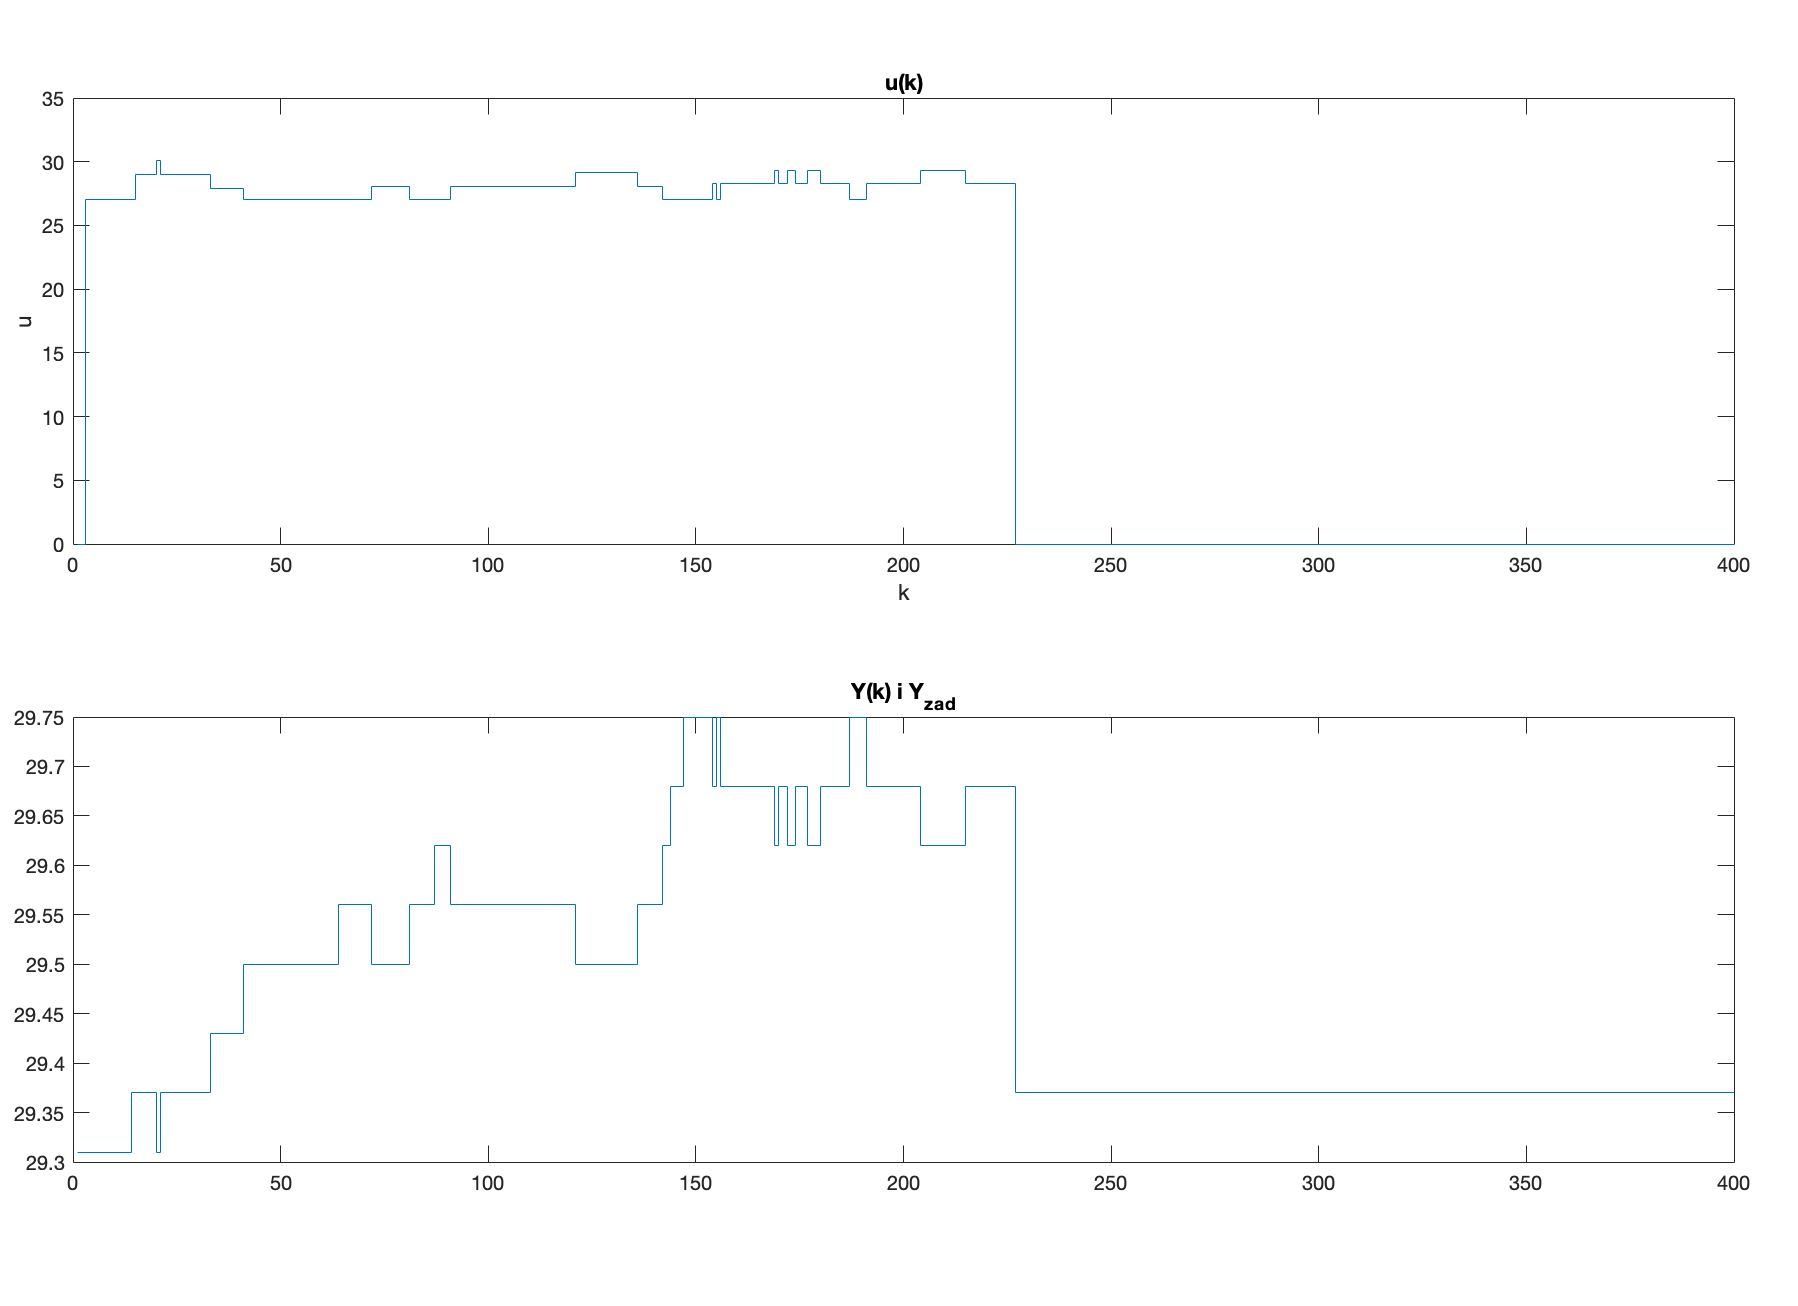
\includegraphics[scale=0.22]{png/lab2/zad5_lab1_pid_k18.png}
	\caption{Przebiegi dla ${K = 18}$ i ${Y_{zad} = 50}$}
	\label{rys_lab_PID_k18}
\end{figure}


\begin{figure}[H]
	\centering
	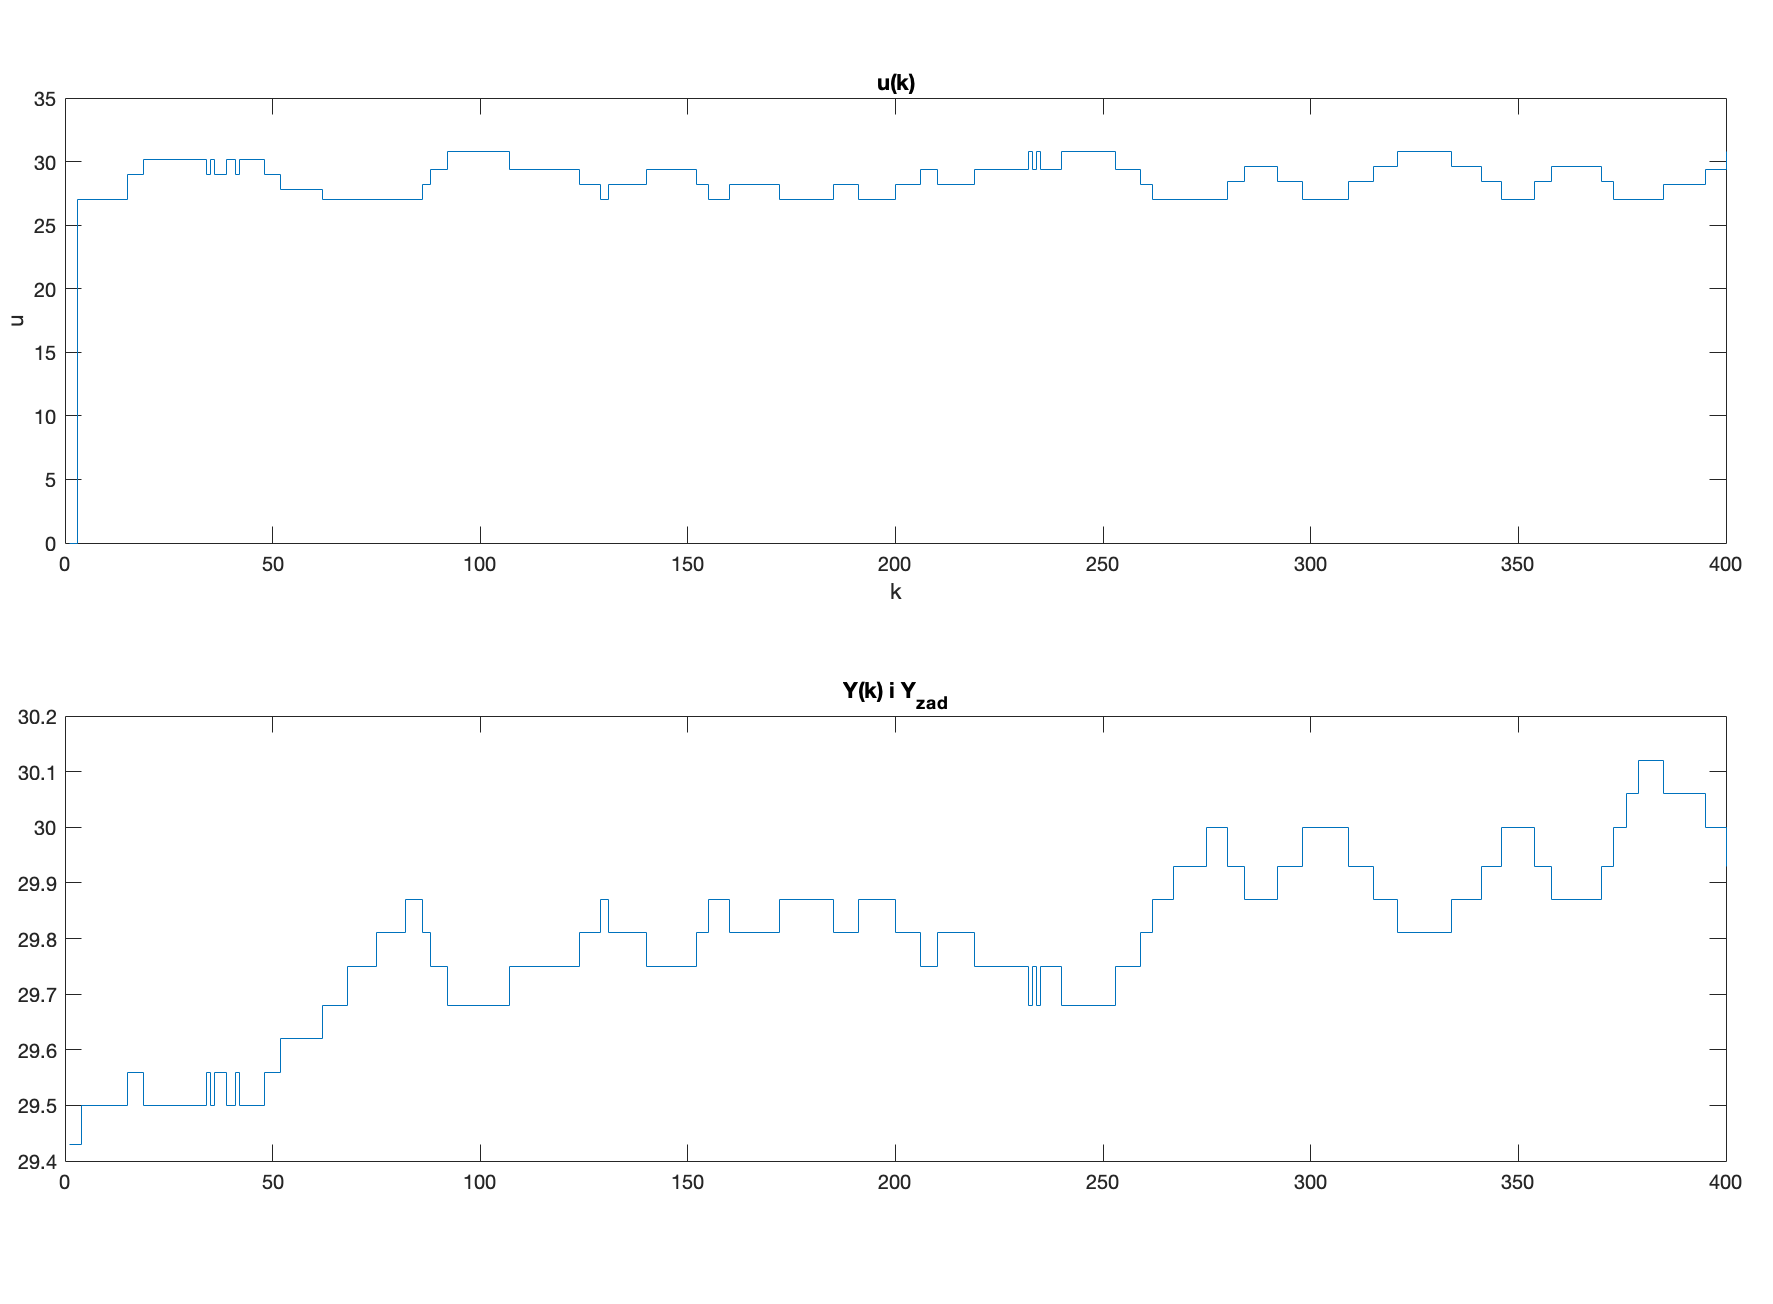
\includegraphics[scale=0.22]{png/lab2/zad5_lab1_pid_k20_v1.png}
	\caption{Przebiegi dla ${K = 20}$ i ${Y_{zad} = 50}$}
	\label{rys_lab_PID_k20_1}
\end{figure}


Po zaobserwowaniu powy�szego problemu i jego analizie zmieniono warto�� sygna�u zadanego na ${Y_{zad} = 33}$. Wyniki widoczne s� na wykresie Rys.  {\ref{rys_lab_PID_k20_2}}.


\begin{figure}[H]
	\centering
	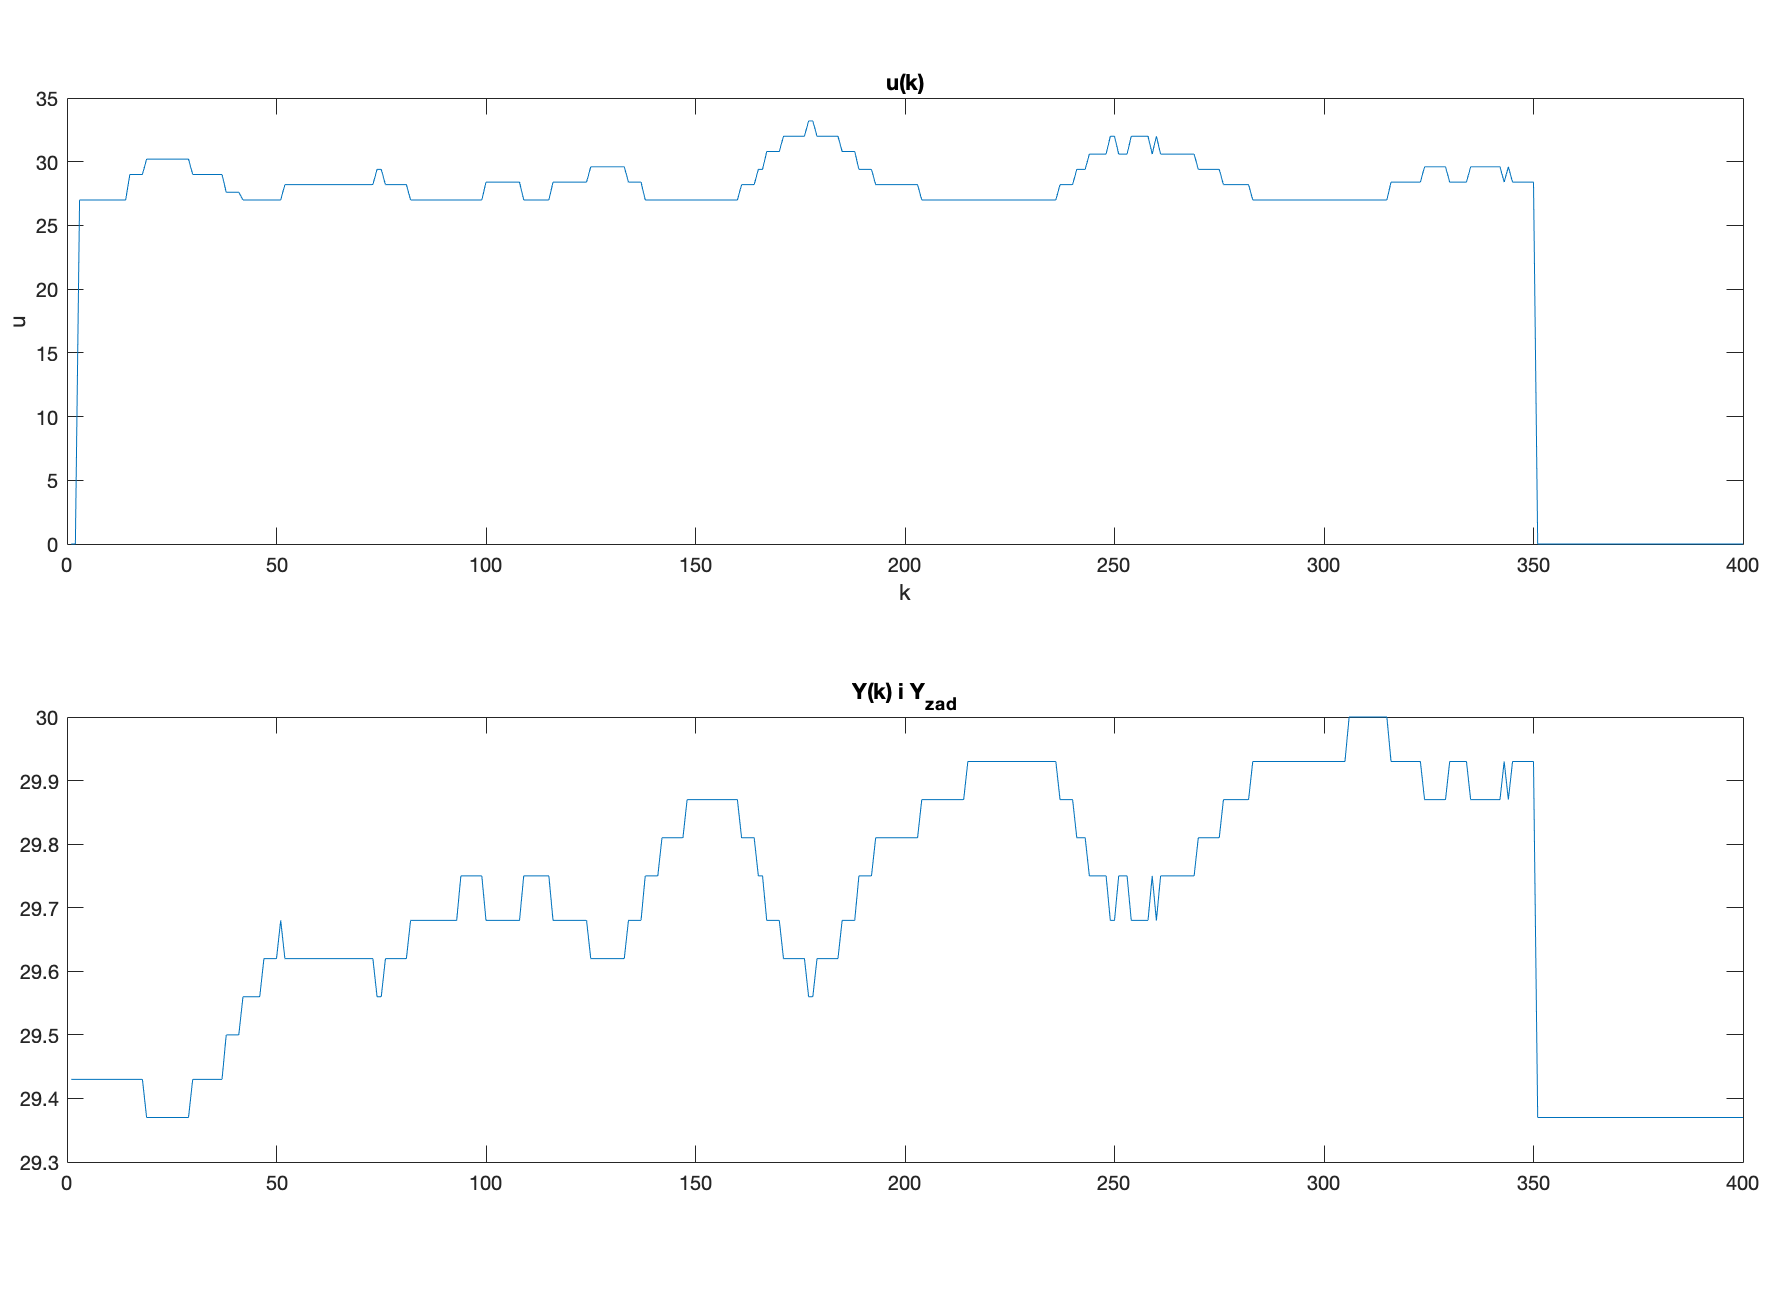
\includegraphics[scale=0.22]{png/lab2/zad5_lab1_pid_k20_v2.png}
	\caption{Przebiegi dla ${K = 20}$ i ${Y_{zad} = 33}$}
	\label{rys_lab_PID_k20_2}
\end{figure}

Mimo tej zmiany, odpowied� procesu nadal ros�a zbyt wolno. Po ponownej analizie algorytmu wywnioskowano, �e do niskiej pr�dko�ci wzrastania przyczyni� si� r�wnie� niew�a�ciwie dobrany parametr ${\Delta U_{max}=2}$ � ogranicza� on bowiem szybko�� zmian sygna�u steruj�cego. Po zmianie tej warto�ci na ${\Delta U_{max} = 20}$, uk�ad dzia�a� zgodnie z za�o�eniami (Rys. {\ref{rys_lab_PID_k20_3}}). 


\begin{figure}[H]
	\centering
	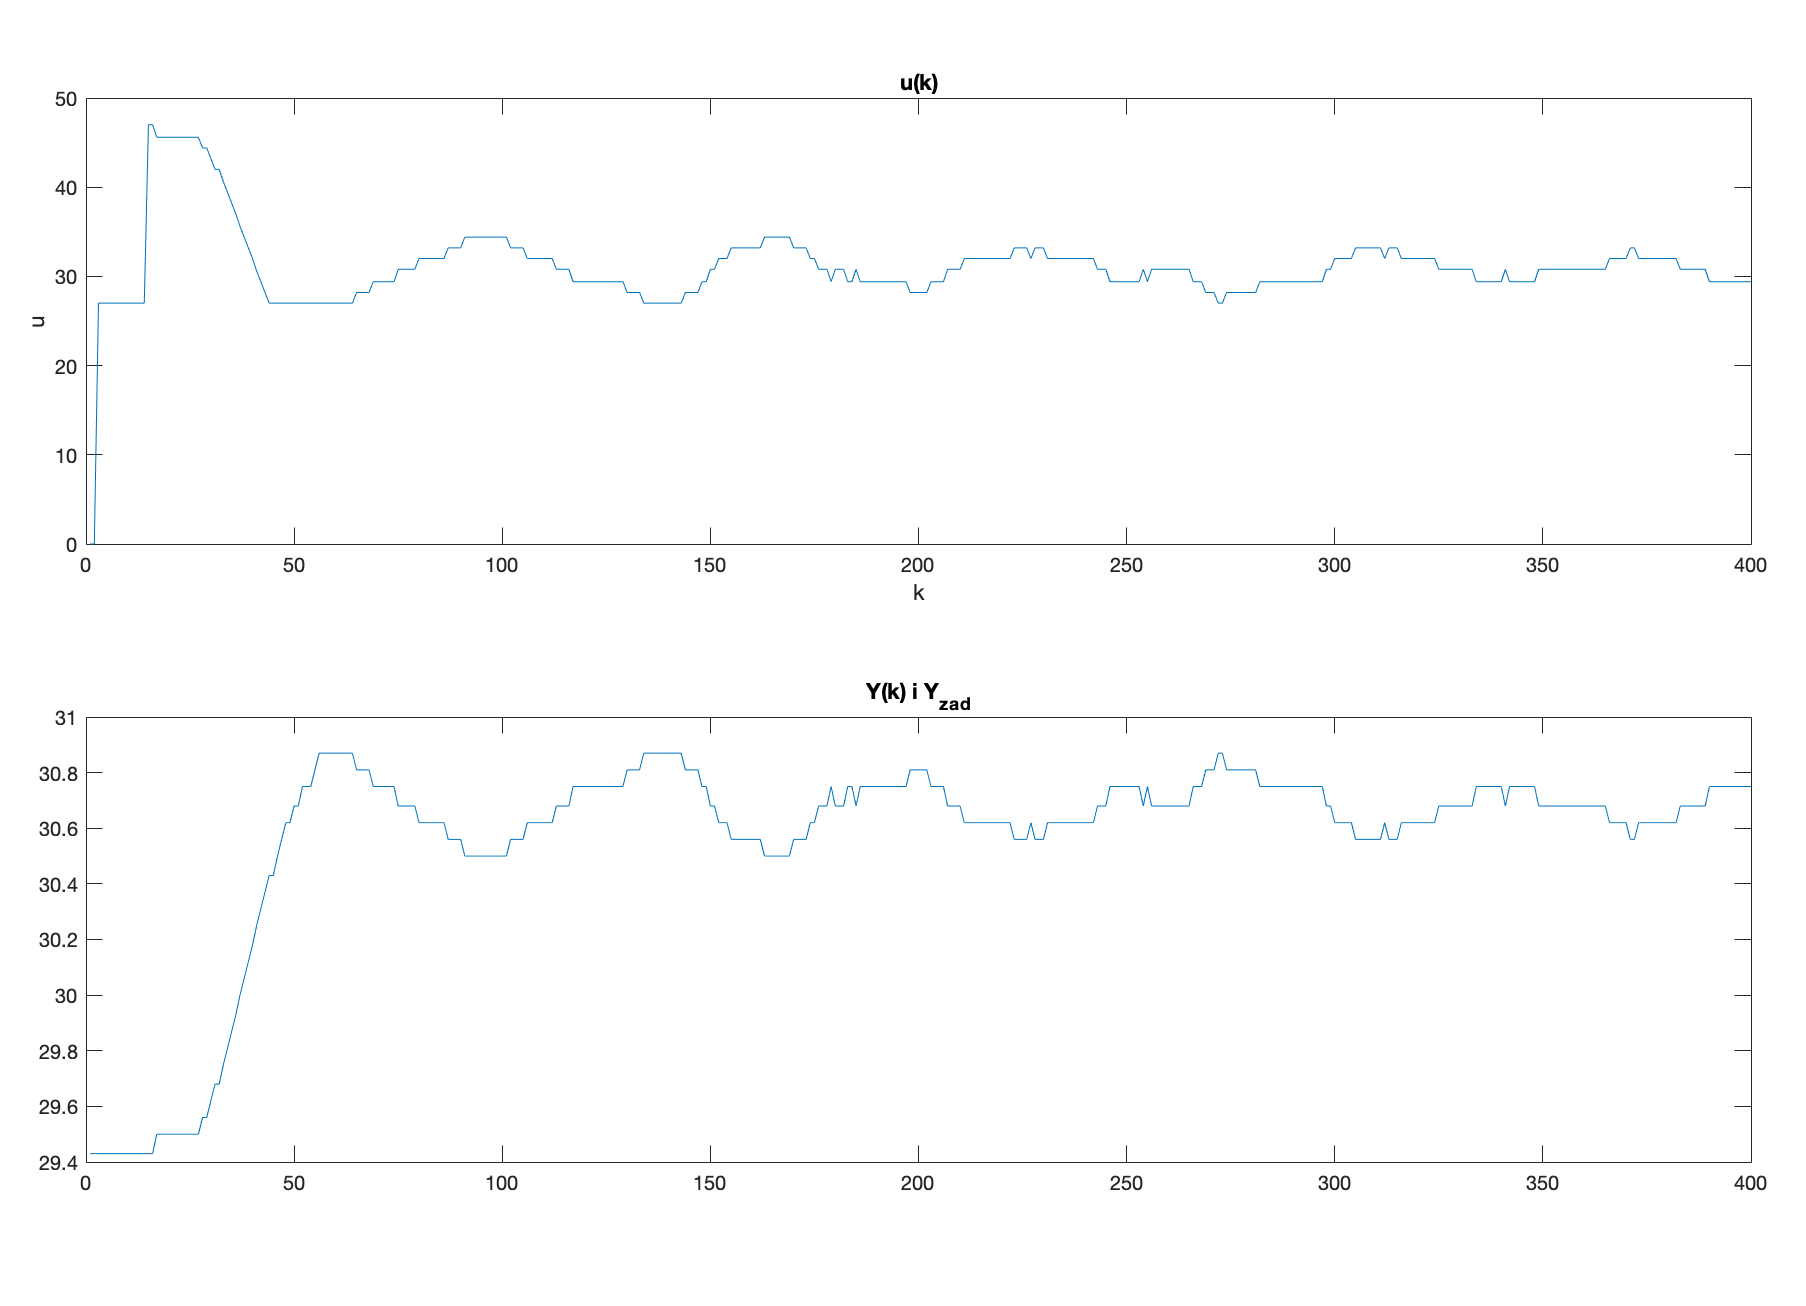
\includegraphics[scale=0.22]{png/lab2/zad5_lab1_pid_k20_v3.png}
	\caption{Przebiegi dla ${K = 20}$, ${Y_{zad} = 33}$ i zmienion� warto�ci� ${\Delta U_{max}}$}
	\label{rys_lab_PID_k20_3}
\end{figure}

Widoczne s� regularne oscylacje, jednak s� one oscylacjami gasn�cymi. Warto�� wzmocnienia zosta�a wi�c zwi�kszona do ${K = 24}$. Jak wida� na wykresie Rys. {\ref{rys_lab_PID_k24}} oscylacje nie gasn�. Zauwa�alny jest  nawet lekki wzrost amplitudy oscylacji. Przewidujemy, �e niegasn�ce oscylacje wyst�pi�yby przy warto�ci wzmocnienia ${K_{kr}=23}$, jednak przez problemy wyst�puj�ce na pocz�tku realizacji zadania nie zosta�o to sprawdzone.
Z tego powodu nie dobrano r�wnie� pozosta�ych parametr�w regulatora PID dla zmiennego sygna�u zadanego. 
Je�li zesp� mia�by wi�cej czasu, nast�pnym krokiem by�oby ustawienie nastaw regulatora wg. regu� Zieglera-Nicholsa (Rys. {\ref{t_ZN}}). Zatem po wyznaczeniu wzmocnienia krytycznego ${K_{kr}}$, z przebiegu warto�ci sterowania odczytany zosta�by okres krytyczny ${T_{kr}}$, a wst�pne nastawy regulatora PID wynosi�yby: ${K=0.6K_{kr}}$, ${T_i= 0.5T_{kr}}$ i ${T_d=0.125K_{kr}}$. Je�eli by�oby to konieczne, regulator zosta�by dostrojony metod� eksperymentaln�.


\begin{figure}[H]
	\centering
	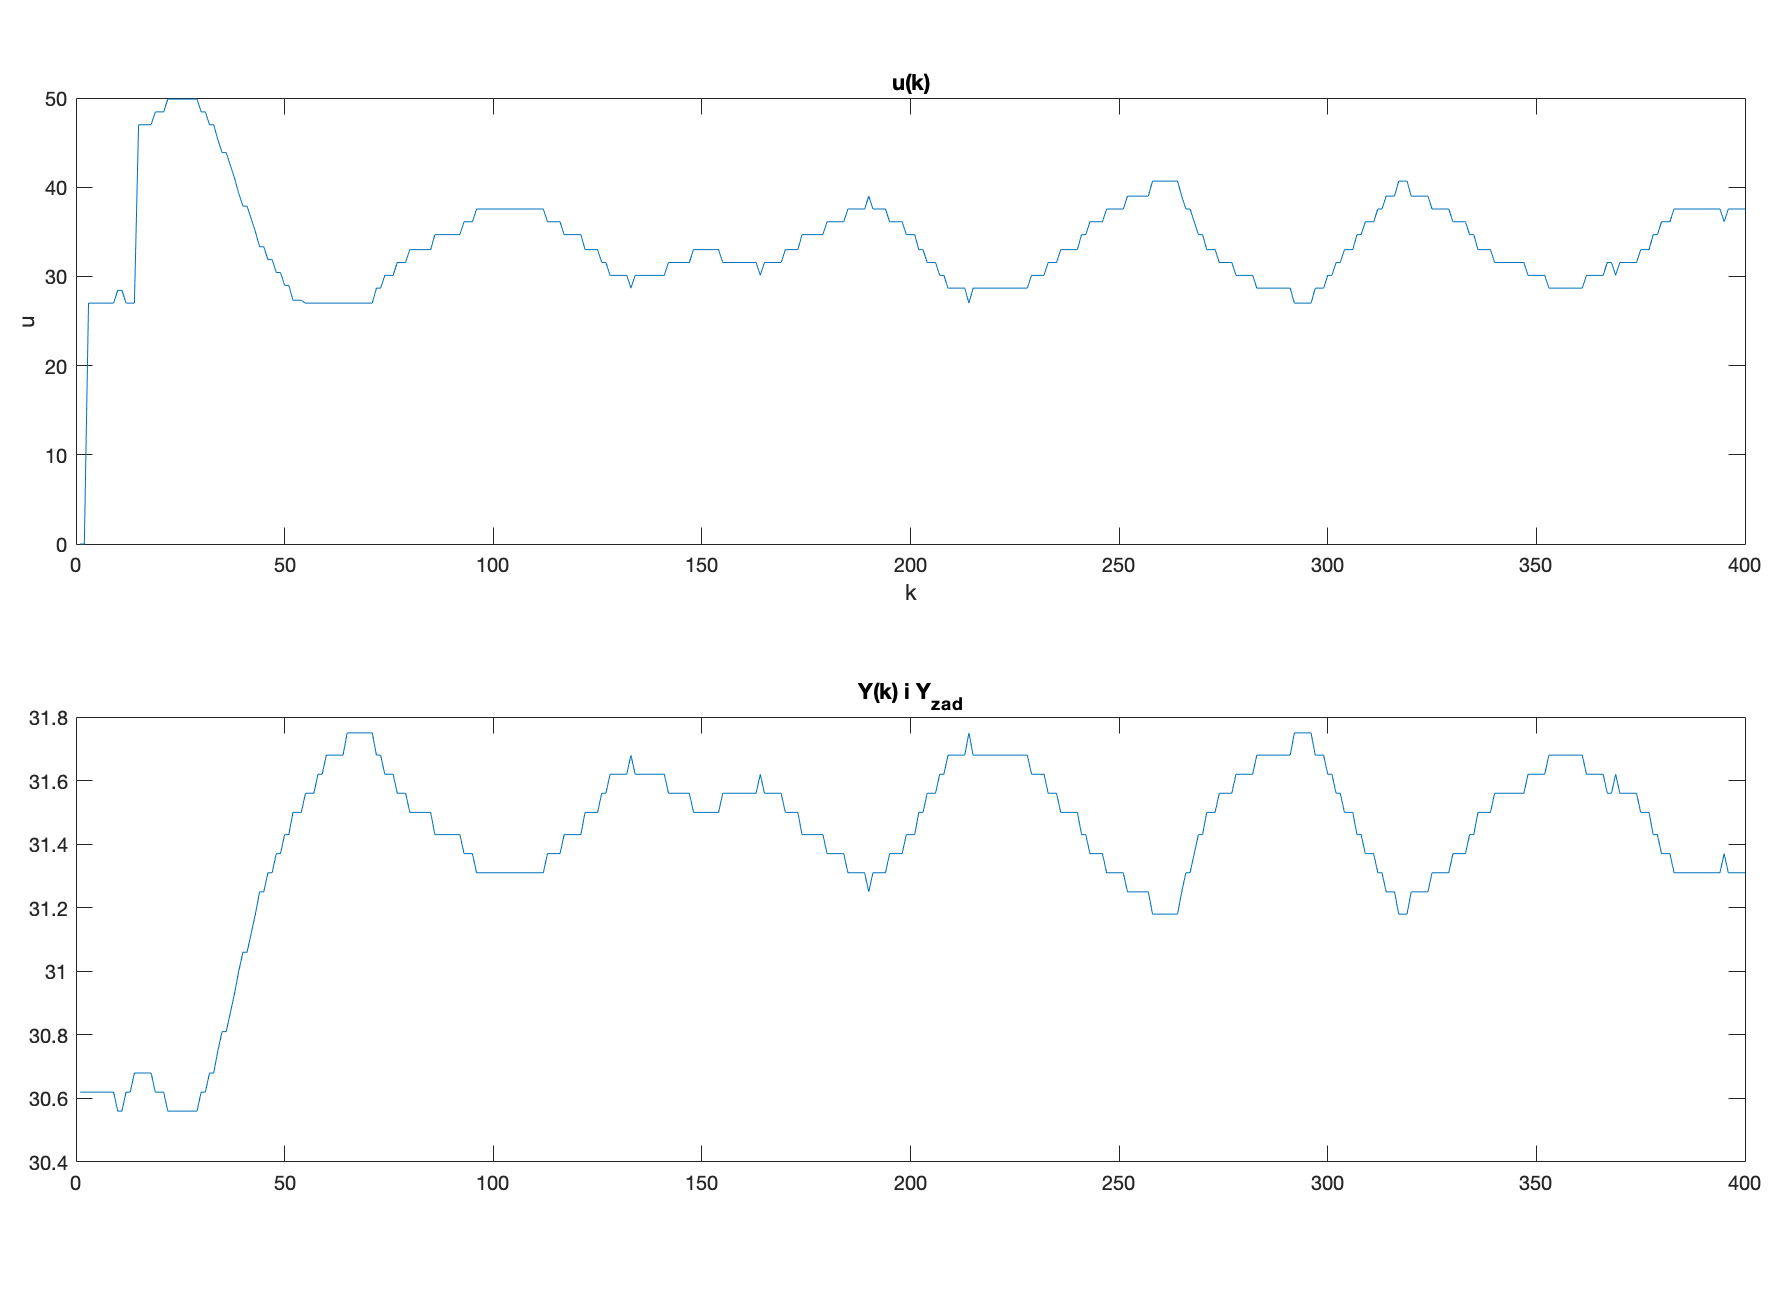
\includegraphics[scale=0.22]{png/lab2/zad5_lab1_pid_k24.png}
	\caption{Przebiegi dla ${K=24}$}
	\label{rys_lab_PID_k24}
\end{figure}



\section{Algorytm DMC}




%% !TEX encoding = cp1250
\chapter{Wzory matematyczne}
Stosujemy przecinek dziesi?tny, a~nie kropk? dziesi?tn?. Aby unikn?? dodatkowego odst?pu, stosujemy zapis \verb+\num{1,2345}+ lub \verb+\num{1.2345}+, co prowadzi do \num{1,2345}, a~nie \verb+$1,2345$+, co prowadzi do $1,2345$. Stosujemy zapis \num{1.2345e10}, a~nie $1{,}2345\times 10^{10}$. Powy?szy zapis mo?na stosowa? r�wnie? w trybie matematycznym, np. \verb+$\num{1.2345e10}$+ skompiluje si? do $\num{1.2345e10}$.

\section{Sta?e i~zmienne, indeksowanie}
Skalarne sta?e i~zmienne zapisujemy w~trybie matematycznym, np. $x$, $y$, $z$. Stosujemy indeksy dolne, np. $x_i$, g�rne, np. $x^j$, lub oba, np. $x_i^j$. Mo?na r�wnie? zastosowa? indeksy w~nawiasach, np. $y(k)$. Je?eli indeks zapisany jest czcionk? pochy??, spodziewamy si?, ?e przyjmuje on warto?? liczbow? (liczby naturalne), np. $x_i$ dla $i=1,\ldots,10$. Je?eli natomiast zastosujemy oznaczenie $x_{\mathrm{i}}$, to w�wczas indeks $\mathrm{i}$ nie przyjmuje ?adnej warto?ci, jest on integraln? cz??ci? zmiennej lub sta?ej. Dlatego oznaczaj?c horyzont sterowania stosujemy symbol $N_{\mathrm{u}}$, a~nie $N_u$, co by sugerowa?o, ?e indeks $u$ przyjmuje pewne warto?ci z zakresu liczb naturalnych. Analogicznie, sta?a czasowa ca?kowania oznaczana jest jako $T_{\mathrm{i}}$, a~nie jako $T_i$, sta?a czasowa r�?niczkowania to $T_{\mathrm{d}}$, a nie $T_d$. Sygna? warto?ci zadanej oznaczamy przez $y^{\mathrm{zad}}$, a~nie przez $y^{zad}$.

Nie nale?y stosowa? czcionki pochy?ej r�wnie? do tekst�w, kt�re uzupe?niaj? wyra?enia matematyczne, np. zamiast b??dnej postaci
\begin{equation}
y(x)=
\begin{cases}
x^2 & gdy \ x\le 0\\
x^3 & gdy \ x>0
\end{cases}
\nonumber
\end{equation}
powinno by?
\begin{equation}
y(x)=
\begin{cases}
x^2 & \textrm{gdy } x\le 0\\
x^3 & \textrm{gdy } x>0
\end{cases}
\nonumber
\end{equation}
Odst?py w trybie matematycznym wymuszamy za pomoc? instrukcji \verb+\+, \verb+\quad+, \verb+\qquad+ itd.

\section{Wektory}
Do oznaczenia wektor�w najcz??ciej stosujemy symbole pogrubione, np. $\boldsymbol{x}$, $\triangle\boldsymbol{u}(k)$. Pami?tamy, ?e w matematyce wektory zawsze s? pionowe. Wektory, kt�rych elementami s? skalary, zapisujemy wi?c jako
\begin{equation}
\triangle\boldsymbol{u}(k)=\left[\triangle u(k|k) \ \ldots \ \triangle u(k+N_{\mathrm{u}}-1|k) \right]^{\mathrm{T}}
\end{equation}
lub w~postaci
\begin{equation}
\triangle\boldsymbol{u}(k)=\left[
\begin{array}{c}
\triangle u(k|k)\\
\vdots\\
\triangle u(k+N_{\mathrm{u}}-1|k)
\end{array}
\right]
\label{w_dUk}
\end{equation}
Je?eli u?ywamy wektor�w, kt�rych elementami sk?adowymi s? inne wektory, najwygodniej zapisa? je pionowo. Np. elementami wektora (\ref{w_dUk}) s? podwektory
\begin{equation}
\triangle u(k+p|k)=\left[
\begin{array}{c}
\triangle u_1(k+p|k)\\
\vdots\\
\triangle u_{n_{\mathrm{u}}}(k+p|k)
\end{array}
\right]
\label{w_dukp}
\end{equation}
gdzie $p=1,\ldots,N_{\mathrm{u}}$. A wi?c ka?dy z~wektor�w (\ref{w_dukp}) ma d?ugo?? $n_{\mathrm{u}}$, wektor (\ref{w_dUk}) ma d?ugo?? $n_{\mathrm{u}}N_{\mathrm{u}}$.

\section{Macierze}
Do oznaczenia macierzy najcz??ciej stosujemy symbole pogrubione, np. macierz dynamiczna w~algorytmie DMC dla procesu o~jednym wej?ciu i~jednym wyj?ciu ma wymiar $N \times N_{\mathrm{u}}$ i struktur?
\begin{equation}
\boldsymbol{G}=\left[
\begin{array}
{cccc}
s_{1} & 0 & \ldots & 0\\
s_{2} & s_{1} & \ldots & 0\\
\vdots & \vdots & \ddots & \vdots\\
s_{N} & s_{N-1} & \ldots &  s_{N-N_{\mathrm{u}}+1}
\end{array}
\right]
\end{equation}
W~przypadku procesu o~$n_{\mathrm{u}}$ wej?ciach i~$n_{\mathrm{y}}$ wyj?ciach ma ona  wymiar $N\times N_{\mathrm{u}}$ i posta?
\begin{equation}
\boldsymbol{G}=\left[
\begin{array}
{cccc}
\boldsymbol{S}_{1} & \boldsymbol{0}_{n_{\mathrm{y}}\times n_{\mathrm{u}}} & \ldots & \boldsymbol{0}_{n_{\mathrm{y}}\times n_{\mathrm{u}}}\\
\boldsymbol{S}_{2} & \boldsymbol{S}_{1} & \ldots & \boldsymbol{0}_{n_{\mathrm{y}}\times n_{\mathrm{u}}}\\
\vdots & \vdots & \ddots & \vdots\\
\boldsymbol{S}_{N} & \boldsymbol{S}_{N-1} & \ldots &  \boldsymbol{S}_{N-N_{\mathrm{u}}+1}%
\end{array}
\right]
\label{w_G}
\end{equation}
gdzie ka?da z~macierzy sk?adowych ma wymiar $n_{\mathrm{y}}\times n_{\mathrm{u}}$
\begin{equation}
\boldsymbol{S}_p=\left[
\begin{array}
{ccc}
s_p^{1,1} & \ldots & s_p^{1,n_{\mathrm{u}}}\\
\vdots & \ddots & \vdots\\
s_p^{n_{\mathrm{y}},1} & \ldots & s_p^{n_{\mathrm{y}},n_{\mathrm{u}}}
\end{array}
\right]
\end{equation}
gdzie $p=1,\ldots,N$. A~wi?c macierz (\ref{w_G}) ma wymiar $n_{\mathrm{y}}N\times n_{\mathrm{u}}N_{\mathrm{u}}$.

\section{Wi?ksze wyra?enia matematyczne}
W~przypadku d?ugich wzor�w nie nale?y korzysta? z~otoczenia \verb+equation+, poniewa? wz�r taki zwykle nie~mie?ci si? na stronie o przyj?tej szeroko?ci, np.
\begin{equation}
y(k)=b_1u(k-1)+b_2u(k-2)+b_3u(k-3)+b_4u(k-4)+b_5u(k-5)-a_1y(k-1)-a_2y(k-2)-a_3y(k-3)-a_4y(k-4)-a_5y(k-5)
\end{equation}
Nale?y zastosowa? otoczenie \verb+align+, co prowadzi do wzoru
\begin{align}
y(k)&=b_1u(k-1)+b_2u(k-2)+b_3u(k-3)+b_4u(k-4)+b_5u(k-5)\nonumber\\
&\quad -a_1y(k-1)-a_2y(k-2)-a_3y(k-3)-a_4y(k-4)-a_5y(k-5)\label{w_yk}
\end{align}
Nie stosujemy otoczenia \verb+split+ z~powodu b??dnego centrowania. Numer wzoru z?o?onego z~wielu wierszy umieszczamy tylko w~ostatnim wierszu.





%% !TEX encoding = cp1250
\chapter{Listingi program�w}
Do zamieszczenia program�w mo?na zastosowa? otoczenie \verb+verbatim+, ale znacznie wi?ksze mo?liwo?ci oferuje pakiet \verb+listings+. Przyk?adowy program w~j?zyku C ma posta?:
\begin{lstlisting}[style=customc,frame=single] 
//Hello World in C
#include <stdio.h>
int main (void)
{
   puts ("Hello World!");
   return 0;
}
\end{lstlisting}
natomiast przyk?adowy program w~j?zyku \verb+MATLAB+ jest nast?puj?cy:
%\begin{lstlisting}[style=custommatlab,frame=single]
\begin{lstlisting}[style=Matlab-editor]
%Hello World in MATLAB
clear all;

disp('Hello World!');
\end{lstlisting} 







%\chapter{Tabele}
W~praktyce bardzo cz�sto nale�y wyr�wna� liczby wzgl�dem cyfr znacz�cych w~poszczeg�lnych kolumnach (czyli przecinek dziesi�tny ma by� we wszystkich wierszach tabeli umieszczony w~tym samym miejscu w~pionie). Do wyr�wnania liczb nale�y wykorzysta� pakiet \verb+siunitx+ (pakiety \verb+rccol+ oraz \verb+dcolumn+ maj� mniejsze mo�liwo�ci). Wszystkie przyk�ady podane w~niniejszym rozdziale wykorzystuj� pakiet \verb+siunitx+. Zwr��my uwag�, �e tytu�y znajduj�ce si� w~pierwszym wierszu wszystkich tabel s� wy�rodkowane (w~obr�bie kolejnych kom�rek).

Je�eli standardowa szeroko�� kolumn jest za ma�a, nale�y w~dowolnym wierszu wstawi� z~obu stron zawarto�ci kom�rki polecenia \verb+\hspace{odleg�o��}+, kt�re zapewniaj� odpowiedni� szeroko��. Modyfikacj� tak� zastosowano w~drugiej kolumnie tab.~\ref{t_wyrownanie_do_znaku_przecinek3}.

Je�eli tabela jest szersza ni� szeroko�� strony, nale�y zastosowa� otoczenie \verb+sidewaystable+ z~pakietu \verb+rotating+, co wykorzystano w~tab.~\ref{t_wyrownanie_do_znaku_przecinek4}.

W~zamieszczonych tabelkach wykorzystano polecenie \verb+\rule+ do wstawienia linii o~zerowej szeroko�ci do wierszy tabelek, kt�re s� zbyt w�skie.

\begin{table}
	[b] \caption{Por�wnanie liczby parametr�w~(LP) i~dok�adno�ci~(SSE) modeli}
	\label{t_wyrownanie_do_znaku_przecinek1}
	\centering
	\sisetup{table-format = 2.4}
	\begin{small}
		\begin{tabular}{|l|S[table-format=2]|S|S|S|}
			\hline
			\multicolumn{1}{|c|}{Model\rule{0pt}{3.5mm}} & LP & $\mathrm{SSE_{ucz}}$ & $\mathrm{SSE_{wer}}$ & $\mathrm{SSE_{test}}$ \\ \hline
			Liniowy \rule{0pt}{3.5mm}                    &  4 & 90.1815              & 70.7787              & \textemdash         \\
			Neuronowy, $K=1$                             &  7 & 10.1649              & 10.3895              & \textemdash         \\
			Neuronowy, $K=2$                             & 13 & 0.3282               & 0.3257               & \textemdash         \\
			Neuronowy, $K=3$                             & 19 & 0.2014               & 0.1827               & 0.1468                \\
			Neuronowy, $K=4$                             & 25 & 0.1987               & 0.1906               & \textemdash         \\
			Neuronowy, $K=5$                             & 31 & 0.1364               & 0.1971               & \textemdash         \\
			Neuronowy, $K=6$                             & 37 & 0.1340               & 0.2044               & \textemdash         \\ \hline
		\end{tabular}
	\end{small}
\end{table}

\begin{table}
	[b] \caption{Por�wnanie liczby parametr�w~(LP) i~dok�adno�ci~(SSE) modeli}
	\label{t_wyrownanie_do_znaku_przecinek2}
	\centering
	\sisetup{table-format = 1.4e-1}
	\begin{small}
		\begin{tabular}{|l|S[table-format=2]|S|S|S|}
			\hline
			\multicolumn{1}{|c|}{Model\rule{0pt}{3.5mm}} & LP & $\mathrm{SSE_{ucz}}$ & $\mathrm{SSE_{wer}}$ & $\mathrm{SSE_{test}}$ \\ \hline
			Liniowy\rule{0pt}{3.5mm} &  4 & 9.1815e1  & 7.7787e1  & \textemdash\\
			Neuronowy, $K=1$         &  7 & 1.1649e1  & 1.3895e1  & \textemdash\\
			Neuronowy, $K=2$         & 13 & 3.2821e-1 & 3.2568e-1 & \textemdash\\
			Neuronowy, $K=3$         & 19 & 2.0137e-1 & 1.8273e-1 & 1.4682e-1\\
			Neuronowy, $K=4$         & 25 & 1.9868e-1 & 1.9063e-1 & \textemdash\\
			Neuronowy, $K=5$         & 31 & 1.3642e-1 & 1.9712e-1 & \textemdash\\
			Neuronowy, $K=6$         & 37 & 1.3404e-1 & 2.0440e-1 & \textemdash\\ \hline
		\end{tabular}
	\end{small}
\end{table}

\begin{table}
	[b] \caption{Por�wnanie z�o�ono�ci obliczeniowej}
	\label{t_wyrownanie_do_znaku_przecinek3}
	\centering
	\sisetup{table-auto-round=true}
	\begin{small}
		\begin{tabular}{|l|S[table-format=2]|S[table-format=1.2]|S[table-format=1.2]|S[table-format=2.2]|S[table-format=2.2]|S[table-format=2.2]|S[table-format=3.2]|}
			\hline
			\multicolumn{1}{|c|}{Algorytm\rule{0pt}{3.25mm}} & \hspace{0.5cm} $N$ \hspace{0.5cm} & ${N_{\mathrm{u}}=1}$ & ${N_{\mathrm{u}}=2}$ & ${N_{\mathrm{u}}=3}$ & ${N_{\mathrm{u}}=4}$ & ${N_{\mathrm{u}}=5}$ & ${N_{\mathrm{u}}=10}$ \\ \hline
			NPL\rule{0pt}{3.5mm} & 5 & 0,3954 & 0,5326 & 0,8482 & 1,2868 & 1,9179 & \textemdash \\
			NO & 5 & 2,6129 & 5,0372 & 8,0029 & 12,6476 & 18,3668 & \textemdash \\
			NO$_{\mathrm{apr}}$\rule[-1.5mm]{0pt}{3.5mm} & \phantom{0}5 & 2,4654 & 4,3206 & 7,9801 & 15,2479 & 26,5298 & \textemdash \\ \hline
			NPL\rule{0pt}{3.5mm} & 10 & 0,6274 & 0, 7874 & 1,1366 & 1,6201 & 2,3101 & 9,1346 \\
			NO & 10 & 5,2040 & 9,0378 & 13,5571 & 19,1675 & 26,2604 & 76,5018 \\		
			NO$_{\mathrm{apr}}$\rule[-1.5mm]{0pt}{3.5mm} & 10 & 4,3828 & 7,5813 & 12,6279 & 20,0911 & 31, 7747 & 154,1544 \\ \hline
		\end{tabular}
	\end{small}
\end{table}

\begin{sidewaystable}
	[b] \caption{Por�wnanie z�o�ono�ci obliczeniowej}
	\label{t_wyrownanie_do_znaku_przecinek4}
	\centering
	\centering
	\sisetup{table-auto-round=true}
	\begin{small}
		\begin{tabular}{|l|S[table-format=2]|S[table-format=1.2]|S[table-format=1.2]|S[table-format=2.2]|S[table-format=2.2]|S[table-format=2.2]|S[table-format=3.2]|S[table-format=3.2]|S[table-format=3.2]|S[table-format=3.2]|}
			\hline
			\multicolumn{1}{|c|}{Algorytm\rule{0pt}{3.25mm}} & $N$ & ${N_{\mathrm{u}}=1}$ & ${N_{\mathrm{u}}=2}$ &
			${N_{\mathrm{u}}=3}$ &
			${N_{\mathrm{u}}=4}$ &
			${N_{\mathrm{u}}=5}$ &
			${N_{\mathrm{u}}=10}$ &
			${N_{\mathrm{u}}=15}$ &
			${N_{\mathrm{u}}=20}$ &
			${N_{\mathrm{u}}=30}$\\
			\hline
			NPL\rule{0pt}{3.5mm} & \phantom{0}5 & 0,3954 & 0,5326 & 0,8482 & 1,2868 & 1,9179 & \textemdash & \textemdash & \textemdash & \textemdash\\
			NO & \phantom{0}5 & 2,6129 & 5,0372 & 8,0029 & 12,6476 & 18,3668 & \textemdash & \textemdash & \textemdash & \textemdash\\
			NO$_{\mathrm{apr}}$\rule[-1.5mm]{0pt}{3.5mm} & \phantom{0}5 & 2,4654 &  4,3206 & 7,9801 & 15,2479 & 26,5298 & \textemdash & \textemdash & \textemdash & \textemdash\\
			\hline
		\end{tabular}
	\end{small}
\end{sidewaystable}

\end{document}

